\documentclass[a4paper]{scrartcl}
\usepackage[utf8]{inputenc}
\usepackage[english]{babel}
\usepackage{graphicx}
\usepackage{lastpage}
\usepackage{pgf}
\usepackage{wrapfig}
\usepackage{fancyvrb}
\usepackage{fancyhdr}

\usepackage[font=footnotesize,labelfont=bf,skip=2pt]{caption}
\usepackage{hyperref}

\pagestyle{fancy}

% Create header and footer
\headheight 27pt
\pagestyle{fancyplain}
\lhead{\footnotesize{Data Storage Paradigms, IV1351}}
\chead{\footnotesize{Project Report, Task 2}}
\rhead{}
\lfoot{}
\cfoot{\thepage\ (\pageref{LastPage})}
\rfoot{}


\title{Project Report, Task 2}
\subtitle{Data Storage Paradigms, IV1351}
\author{Vincent Ferrigan ferrigan@kth.se}
\date{\today}

\begin{document}
\maketitle
    
% \section*{Tips for Report Writing}
% \textbf{REMOVE THIS SECTION BEFORE SUBMITTING THE REPORT.}\\

% \noindent \textit{The target audience has exactly the same skills as the author,
% except they do not know anything at all about the specific application described
% in the report.} \\

% Consider the following:

% \begin{itemize}
%   \item \textbf{The report must be \textit{centered around the requirements}.
%   Which are they (Introduction), how did you work to meet them (Method), what is
%   the solution that meets them (Result), and how can you be sure they are met
%   (Discussion). This is the IMRaD method.} The requirements on the Introduction,
%   Method, Result and Discussion chapters are described below under each chapter.

%   \item Is spelling and grammar correct? Is spoken language avoided?

%   \item Does the report have a good structure with sections, subsections and
%   paragraphs?

%   \item Is the text clarified with images and/or other figures, and with links
%   to the code in your Git repository? Remember that all figures (images, tables,
%   graphs, code listings, etc) shall be numbered and have a short explaining
%   text.
% \end{itemize}

\section{Introduction}
The assignment involved creating a 
\emph{Logical and Physical Model} 
for the 
\emph{Soundgood music school} 
database. 

However, the primary objective was to create a database that encapsulates the
informational requirements outlined in the provided description. This entails
the implementation of a relational database system along with the utilization of
SQL as the query language.


The author collaborated with
\emph{Elin Blomquist}
when constructing the ''Logical-Physical'' model described in this report.
% \textbf{This chapter tells \textit{what} are you going to do.} 

% Explain the task and the requirements on the solution. It's important to clearly
% state the requirements. \textit{Also specify which other student you worked with
% when solving the tasks, or if you worked alone.} 

\section{Literature Study}
Both the pre-recorded lectures on
\href{https://canvas.kth.se/courses/43013/pages/logical-and-physical-models}{logical and physical models},
given by the course examiner, and the lecture on
\href{https://canvas.kth.se/courses/43013/pages/normalisation}{normalisation} were reviewed,

Chapters 14, 15 and section 9.1 in the main textbook
(Fundamentals of Database Systems) as well as chapter 7 in the
alternative textbook (Database System Concepts) were examined.
Additionally, the document
\href{https://canvas.kth.se/courses/43013/files/7096103?wrap=1}{tips-and-tricks-task2.pdf}
was studied.
The project group relied on the textbook Databasteknik, written by
Thomas Pardon-McCartny and Tore Risch to solve the task at hand.

\clearpage
\section{Method}
\label{sec:method}
% \textbf{This chapter tells \textit{how} you solved the task.}
% Explain how you worked when solving the tasks and how you evaluated that your
% solution met the requirements. \textit{Do not explain your solution and do not
% refer to code}, that belongs to the \textit{Result} chapter. More specific
% instructions for the content can be found under each task on the Project page in
% Canvas.


\subsection*{Tools}
The modeling tool used was \emph{Lucidchart}.
It was chosen to enable version control (through Lucidchart's \emph{Revision History}),
collaborative document sharing, and LucidCharts support for and integration with
\emph{PostgreSQL}.

This report was also written in plain text mode -- \LaTeX.

All code was written in \emph{Visual Studio Code}.
Quick-fixes and editing was, however, done in \emph{Vim}. 
\emph{GIT} and \emph{GitHub} was used for version control.

\subsection*{The overall Work-flow}
To create a \emph{Logical and Physical Model} out of the
\emph{Conceptual Model} (designed during the previous assignment),
the project group performed the following 11 steps:
\begin{enumerate}
  \item Made tables of all entities in the conceptual model.
  \item Turned all single-valued attributes into columns in the tables.
  \item Handled multi-valued attributes, for example, by turning them into separate tables.
  \item Assigned column types, such as \texttt{VARCHAR(100)}.
  \item Added column constraints.
  \item Created primary keys for strong entities.
  \item Established all one-to-one and one-to-many relations.
  \item Created many-to-many relations, for instance, by making cross-reference tables.
  \item Made primary keys and foreign keys for multi-valued attribute tables.
  \item Performed normalization.
  \item Verified that all operations could be performed.
\end{enumerate}

\pagebreak
\section{Result}
The scripts and models for the entire project can be found on GitHub:

\subsubsection*{GitHub-Repo}
\url{https://github.com/VincentFerrigan/kth-iv1351-data-storage-paradigms}

\subsubsection*{The logical and Physical Model}

% \textbf{This chapter explains \textit{the result} of what you did.}

% \textbf{The report must show that you have done the work yourself and that you
% have understood what you have done}, both of these goals are met by carefully
% explaining your solution here in the result chapter, and proving that it meets
% the requirements. \textit{State each requirement that is met} and explain
% \textit{how you met it}. Also include links to your code in your Git
% repository, and include also diagrams, see Figure \ref{fig:diag}, and other
% figures to illustrate your reasoning. All figures must be referenced in the
% text. Ask yourself if the solution is clearly explained, and if the reader
% will understand the application. What would you yourself want to know if you
% read about the application, is that included in the report? More specific
% instructions for the content can be found under each task on the Project page
% in Canvas. 

\begin{figure}[h!]
  \begin{center}
    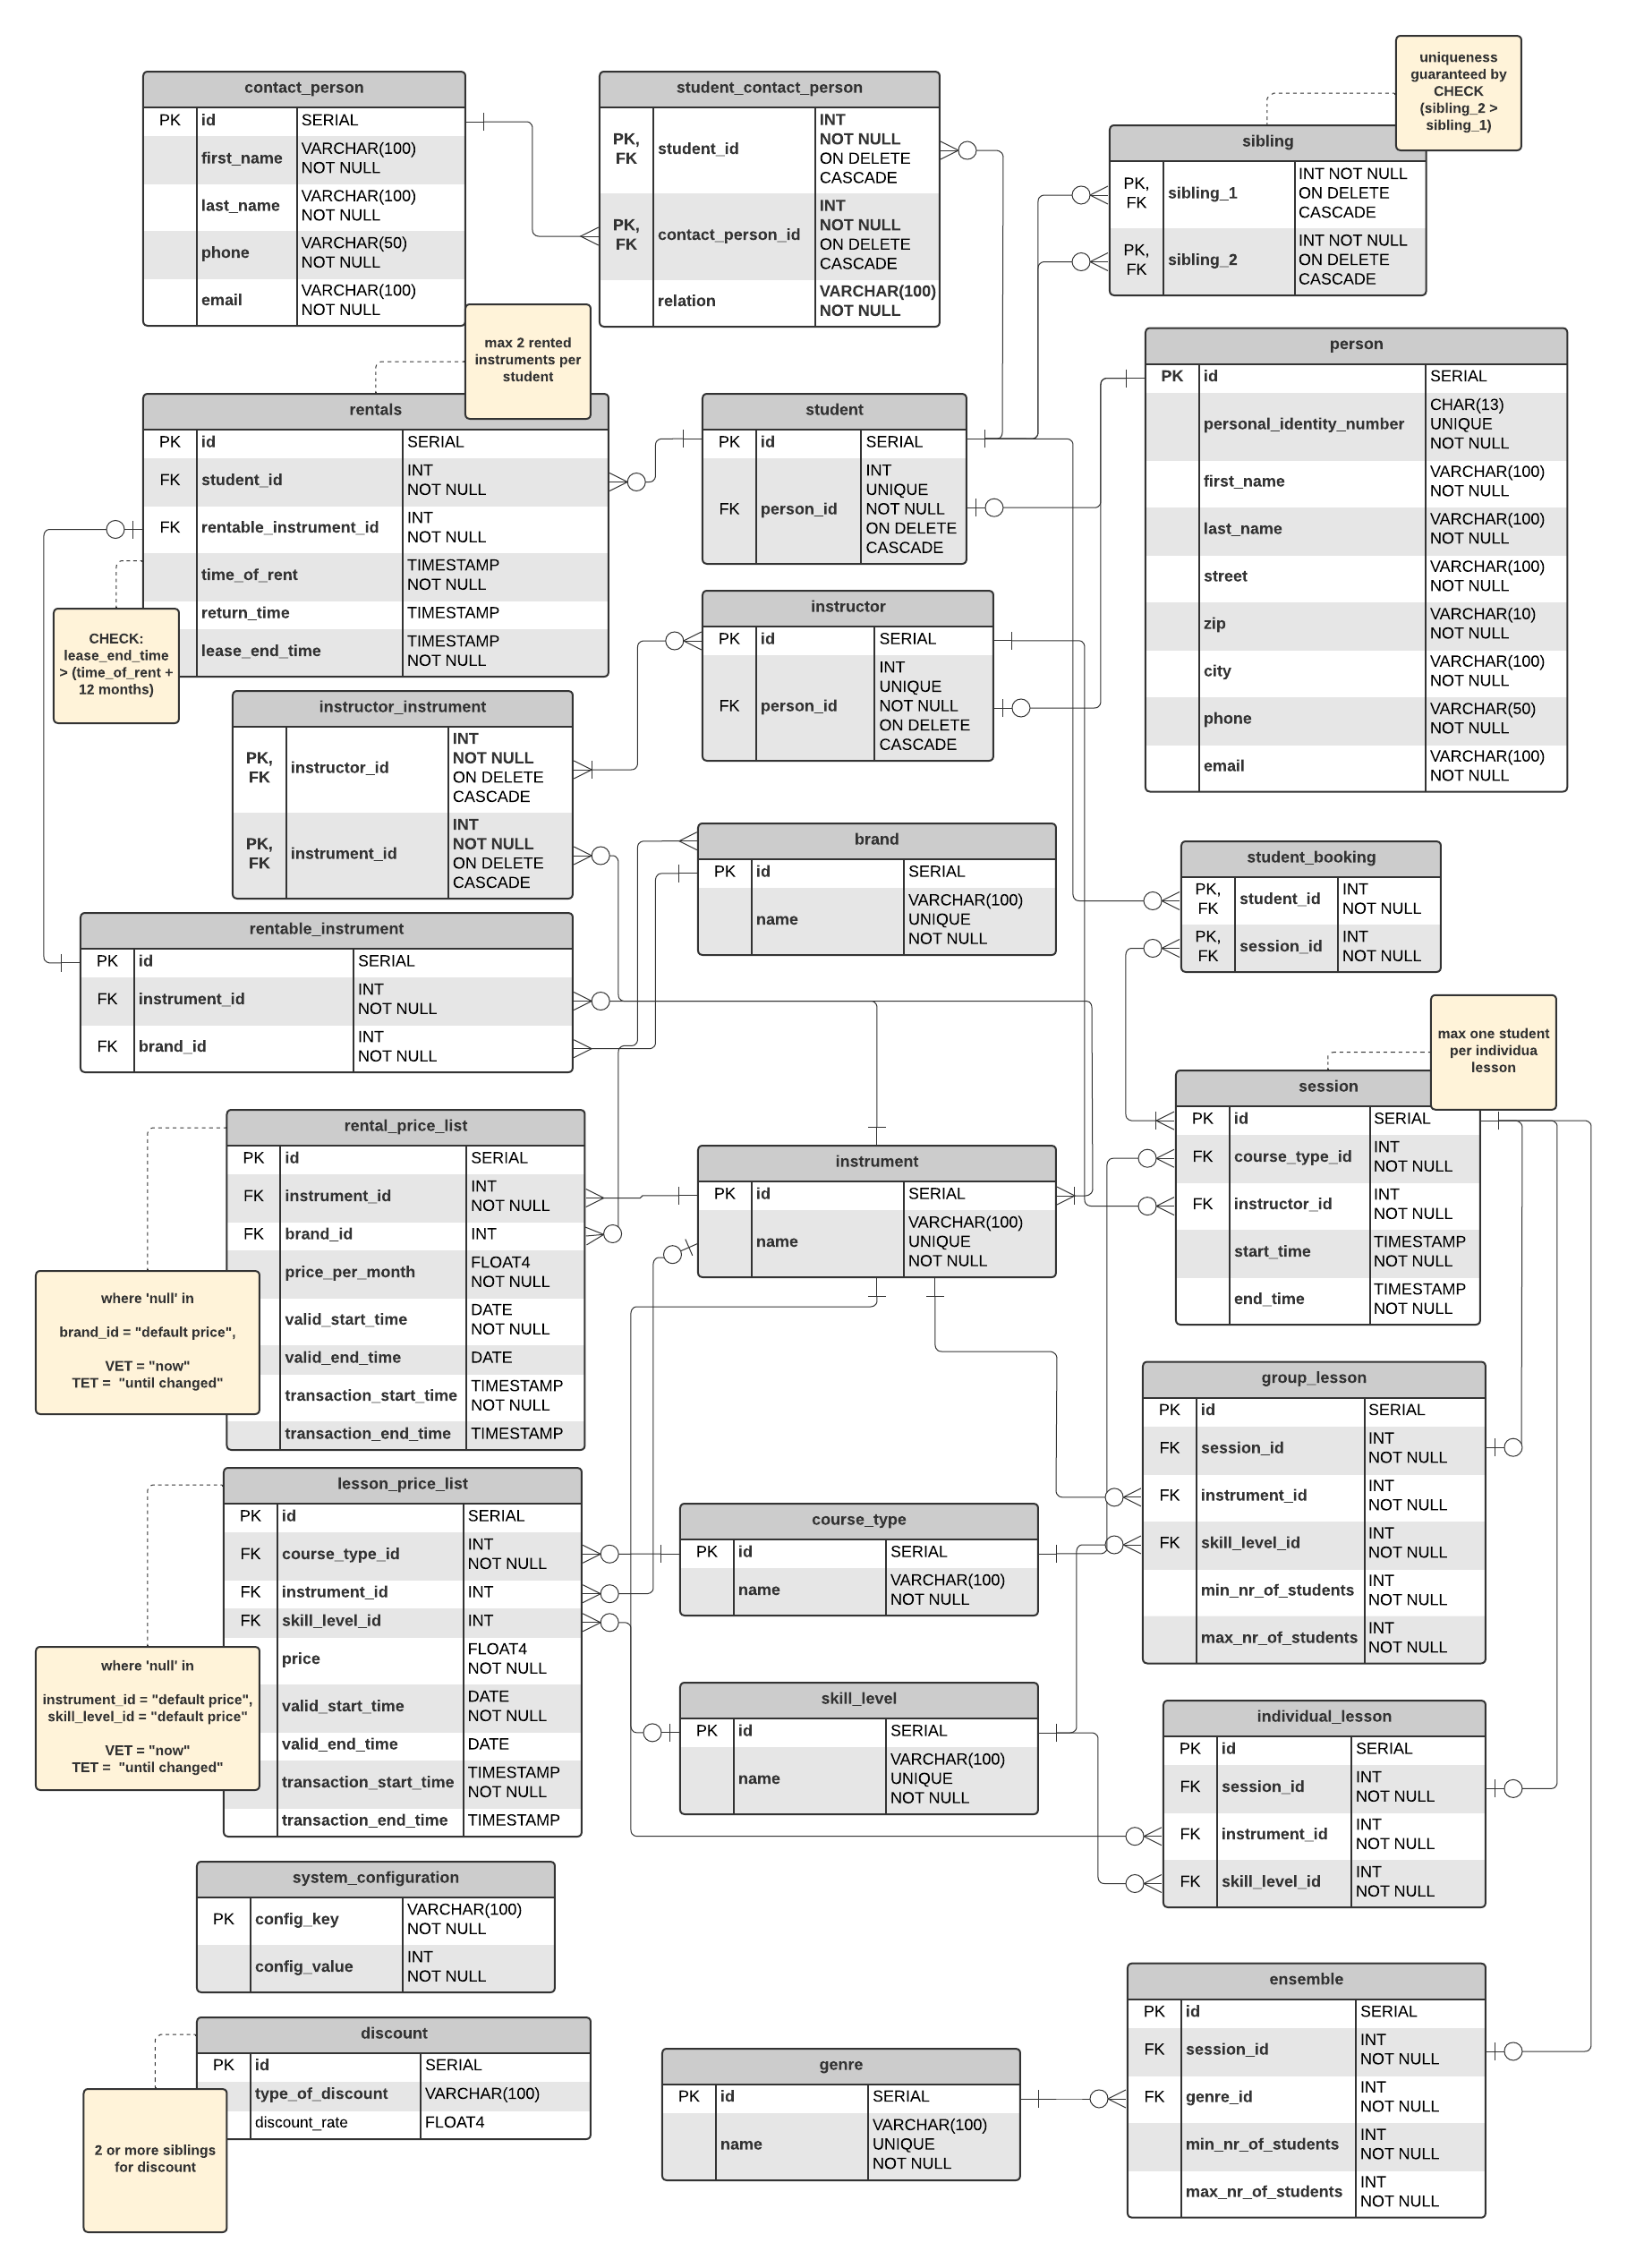
\includegraphics[width=\textwidth]{../figures/logi_phys.png}
    \caption{The Conceptual Model drawn as an ERD using IE notation}
    \label{fig:cm}
  \end{center}
\end{figure}

% VF:
% The naming convention is based on 
% Mozilla's SQL Style Guide. 

% Therefore, \emph{Snake Case}
% (sometimes referred to as underscore case or 
%  snake\_case)
% is used, where each space is replaced with an underscore
% and all letters, including the first letter, is written in lowercase. 

% \begin{figure}[h!]
%   \begin{center}
%     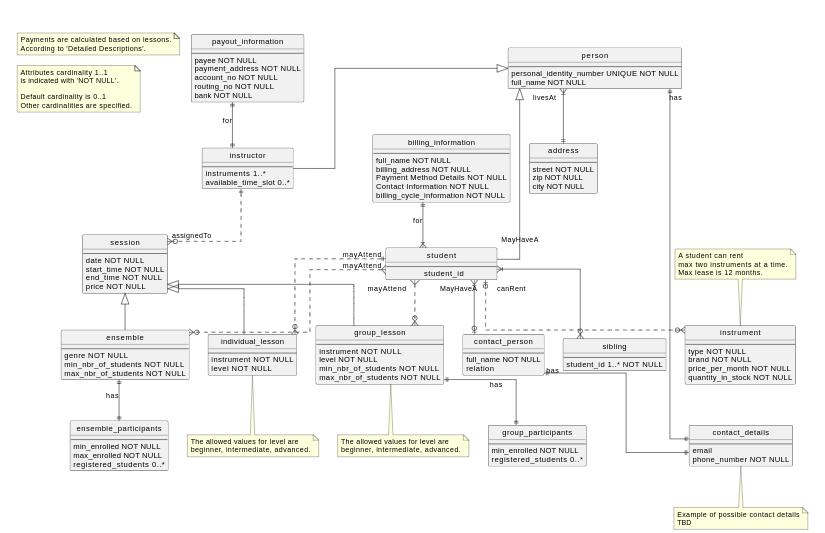
\includegraphics[width=\textwidth]{../figures/i_model.png}
%     \caption{The Conceptual Model with inheritance and payout-/billing information}
%     \label{fig:cm_i}
%   \end{center}
% \end{figure}


\section{Discussion}

% \textbf{This chapter \textit{analysis} the result presented in the previous section.} 

% Evaluate your solution according to the assessment criteria found in the assessment-criteria documents, which are found under the bullet \textit{In the Discussion chapter of your report...}, under each task on the Project page in Canvas. You do not have to cover all specified criteria.

\end{document}
